\section{Alternatives to the $\alpha_{T}$ approach}

Typical observables that separate SUSY signal from the background are $MH_{T}$ and $MH_{T}/H_{T}$. We repeat the same analysis as for the $R_{\alpha T}$ case. We estimate a cut value on $MH_{T}$ at 200 GeV which rejects (mainly) the QCD and $b\bar{b} + \textrm{jets}$ background, while this has a small impact on the SUSY signal. For the $MH_{T}/H_{T}$ observable, a cut value with similar effects is $0.4$. We then calculate the ratio $R_{MHT}$ and $R_{MHT/HT}$.  

Figure \ref{fig:app1} shows the $R_{MHT}$ versus the $|\eta|$ of the leading jet for the SM background only case, in three different $H_{T}$ bins. The dependence on $H_{T}$ value and $|\eta|$ of the leading jet is apparent. In figures~\ref{fig:app2}, we plot the $R_{MHT}$ value for the SUSY signal LM0 (left) and LM1 (right) respectively, plus the SM background, versus the $|\eta|$ of the leading jet. Again the signal case is more central than the background and clearly depends on the $H_{T}$ bin. 

The corresponding plots for $R_{MHT/HT}$ are plotted in figures ~\ref{fig:app3} and ~\ref{fig:app4}. The SM background case is quite similar to the $R_{\alpha T}$ case. The $R_{MHT/HT}$ has a small trend to more central values for higher HT bins. From the background-plus-signal plots, we conclude that $R_{MHT/HT}$ depends highly on the $H_{T}$ and the leading jet $\eta$. 

\begin{figure}[h!]
%\begin{minipage}[b]{0.5\linewidth} % A minipage that covers half the page
\centering
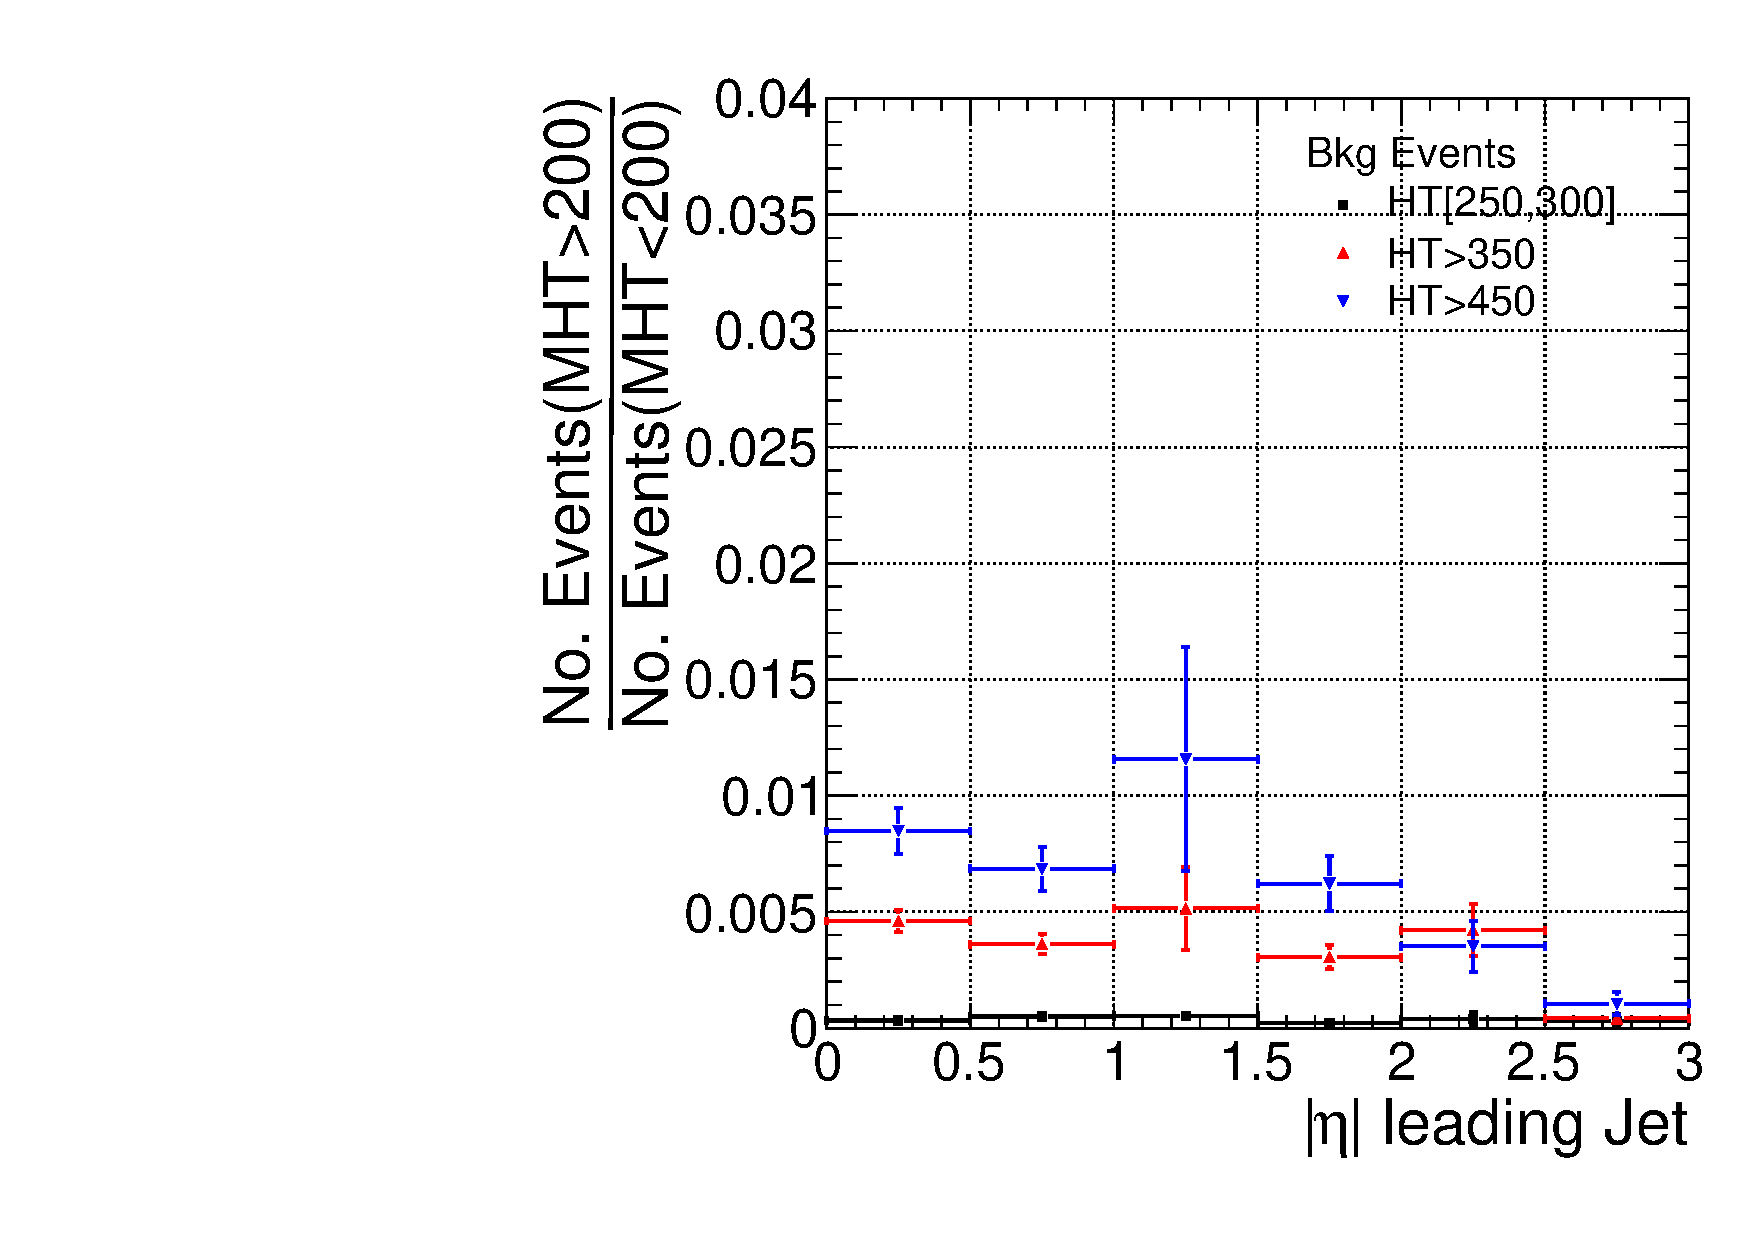
\includegraphics[scale=0.4]{./plots/MHT-NT7-Bkg-MCerr}
%\end{minipage}
%\hspace{0.1cm} % To get a little bit of space between the figures
%\begin{minipage}[b]{0.5\linewidth}
%\centering
%\includegraphics[scale=0.4]{}
%\end{minipage}
\caption{\textit{The $R_{MHT}$ versus the leading jet $|\eta|$ for the SM background-only hypothesis, in three $H_{T}$ bins [250, 350], [350, inf], [450, inf].} }
\label{fig:app1}
\end{figure}

\begin{figure}[h!]
\begin{minipage}[b]{0.5\linewidth}
\centering
{\label{fig:aT}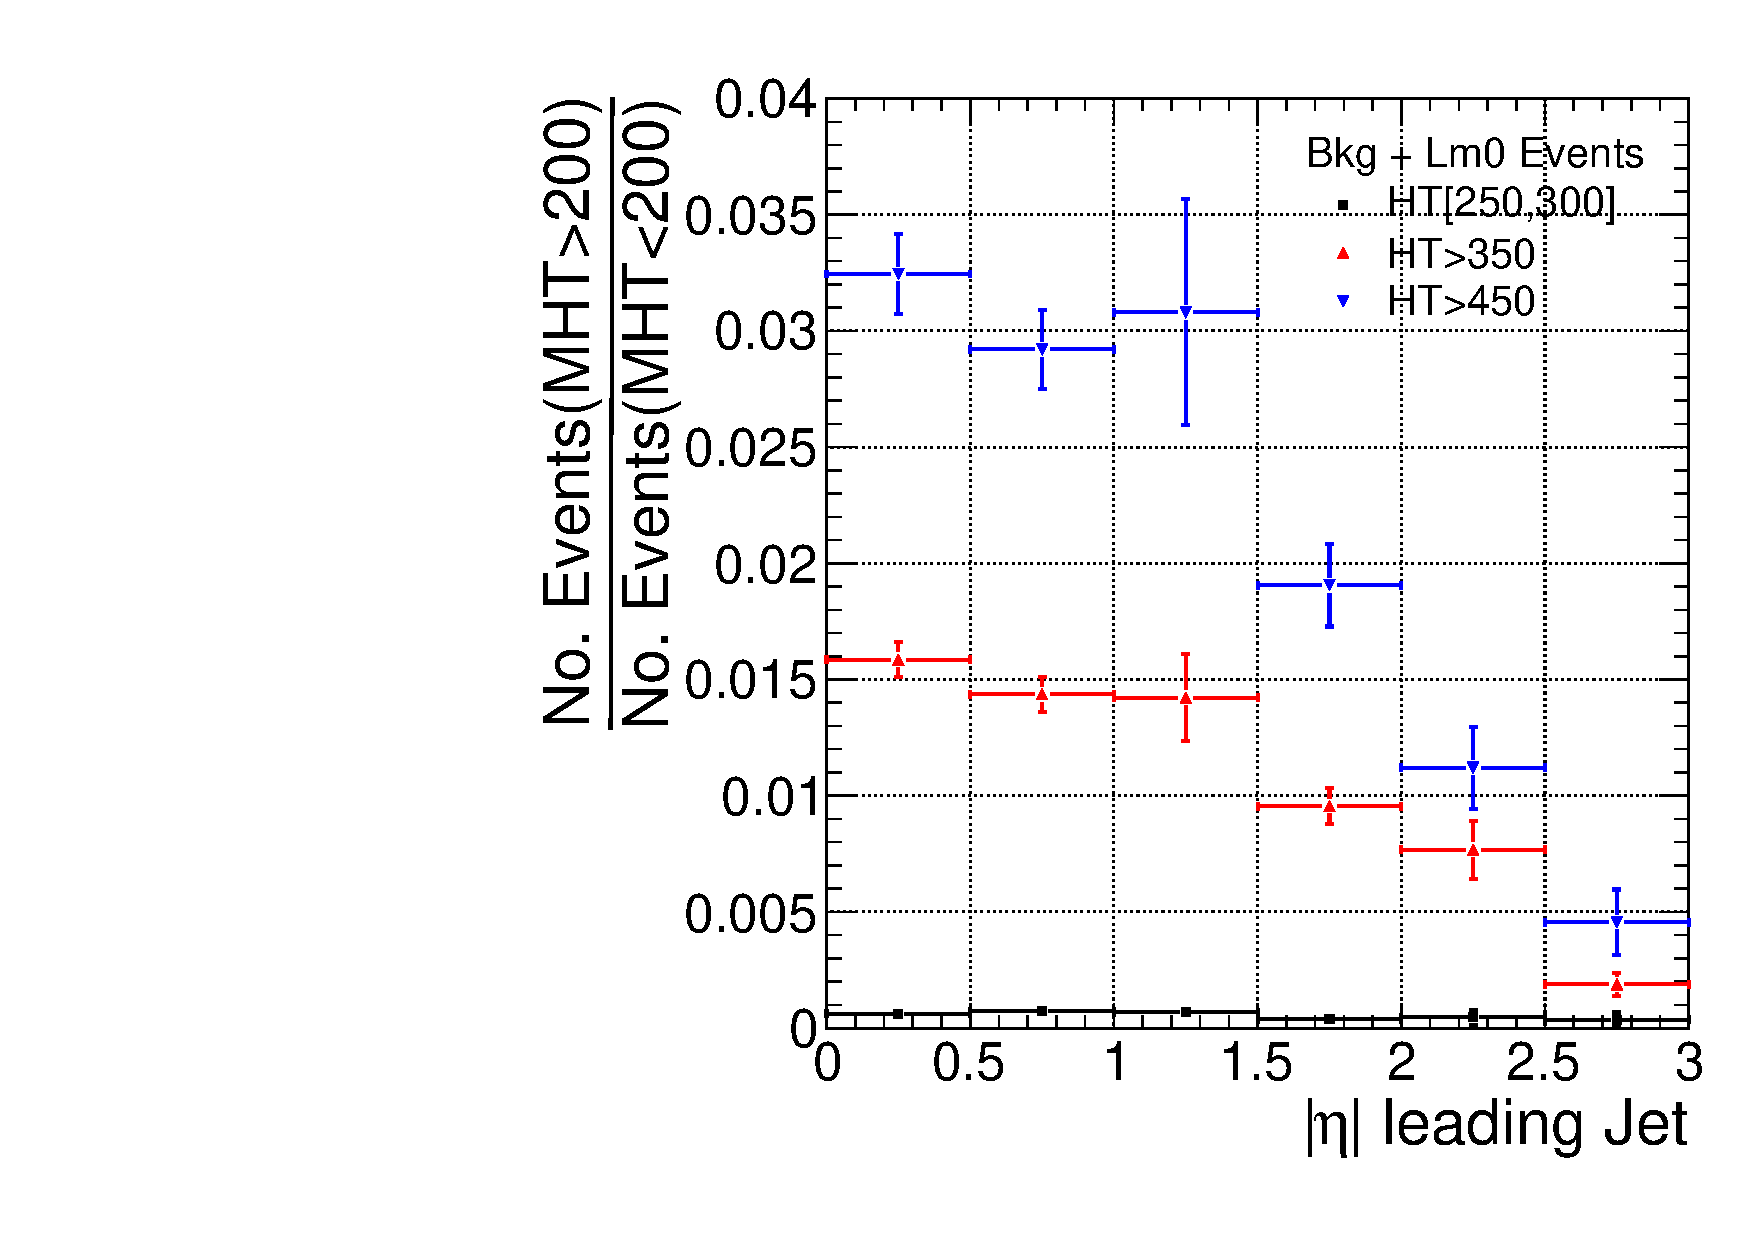
\includegraphics[scale=0.4]{./plots/MHT-NT7-Lm0-MCerr}} 
\end{minipage}
\begin{minipage}[b]{0.5\linewidth}
\centering
{\label{fig:mht}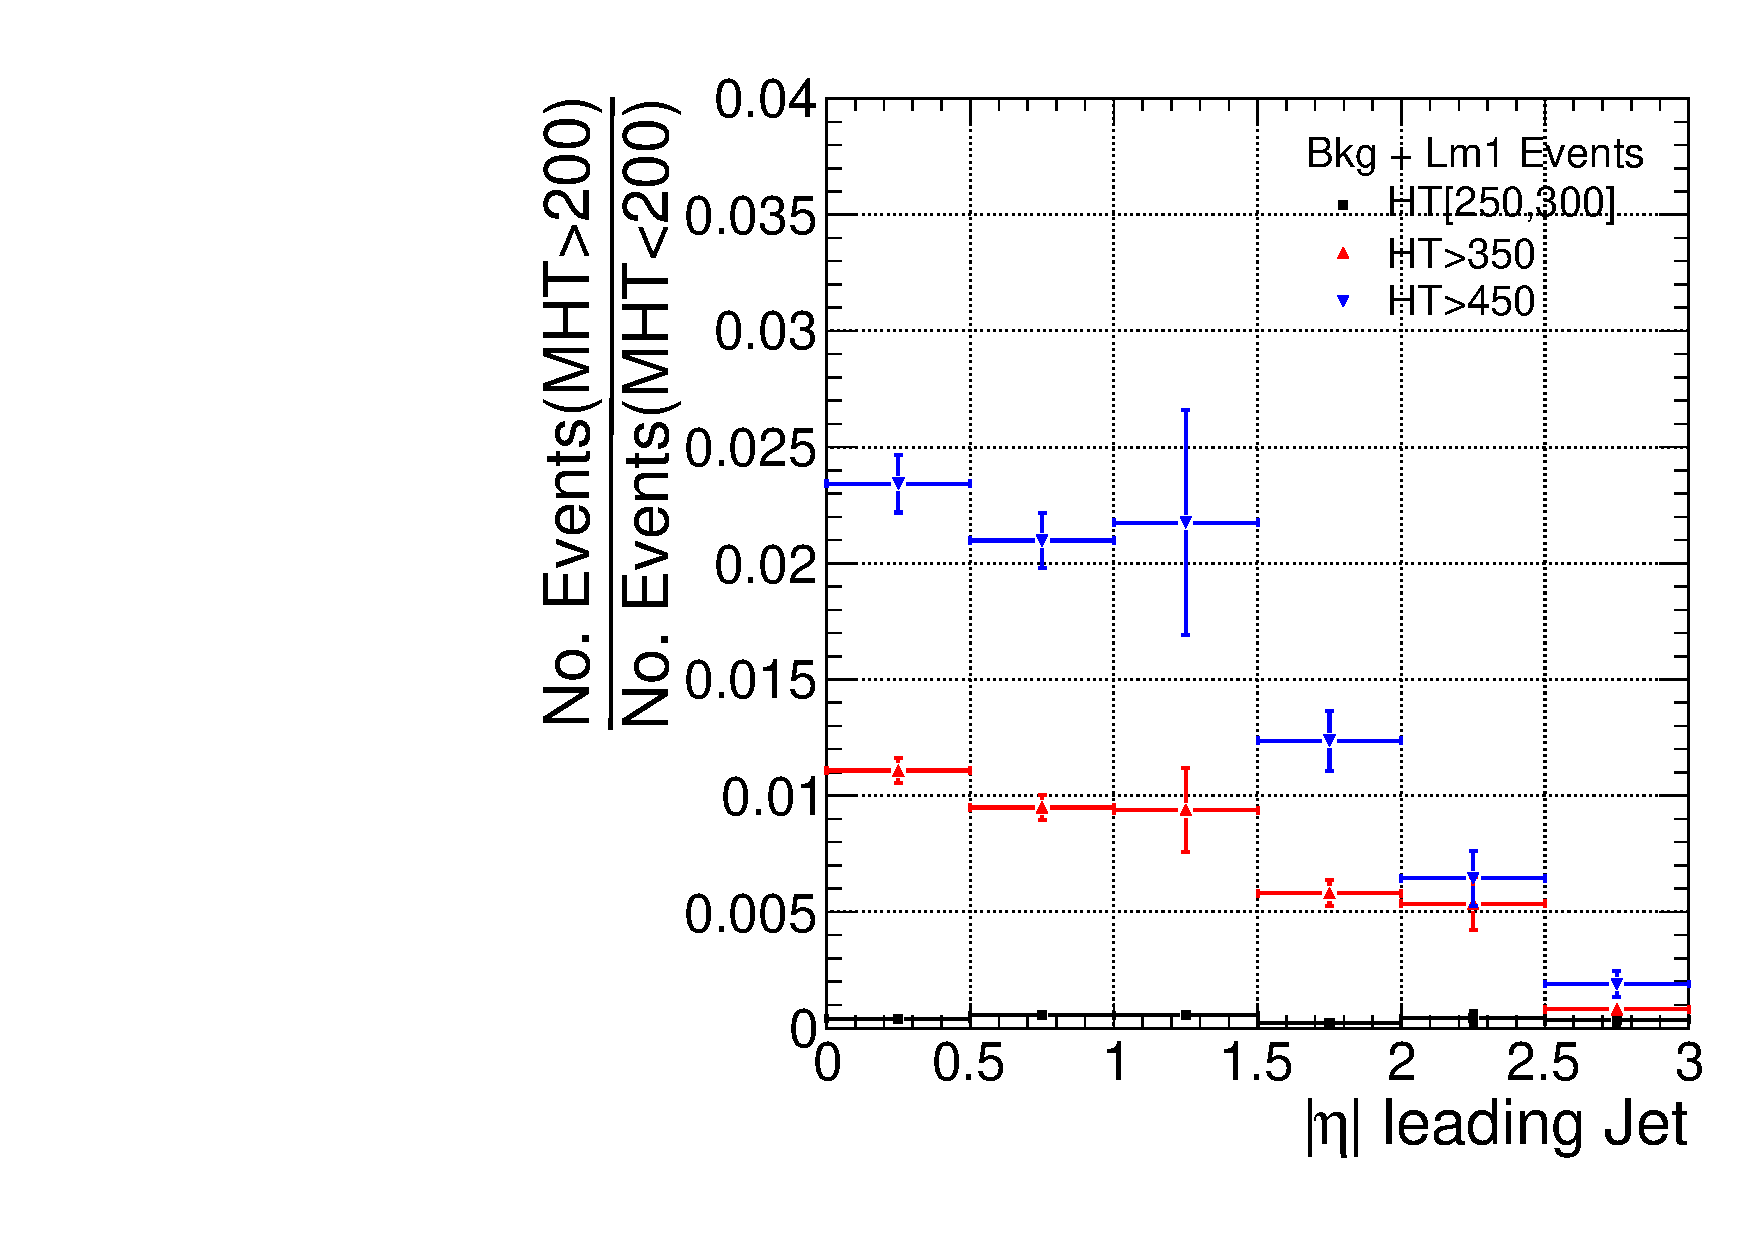
\includegraphics[scale=0.4]{./plots/MHT-NT7-Lm1-MCerr}} 
\end{minipage}
\caption{\textit{The $R_{MHT}$ versus the leading jet $|\eta|$ for the SUSY signal plus SM background hypothesis, in three $H_{T}$ bins [250, 350], [350, inf], [450, inf].} }
\label{fig:app2}
\end{figure}

\begin{figure}[h!]
%\begin{minipage}[b]{0.5\linewidth} % A minipage that covers half the page
\centering
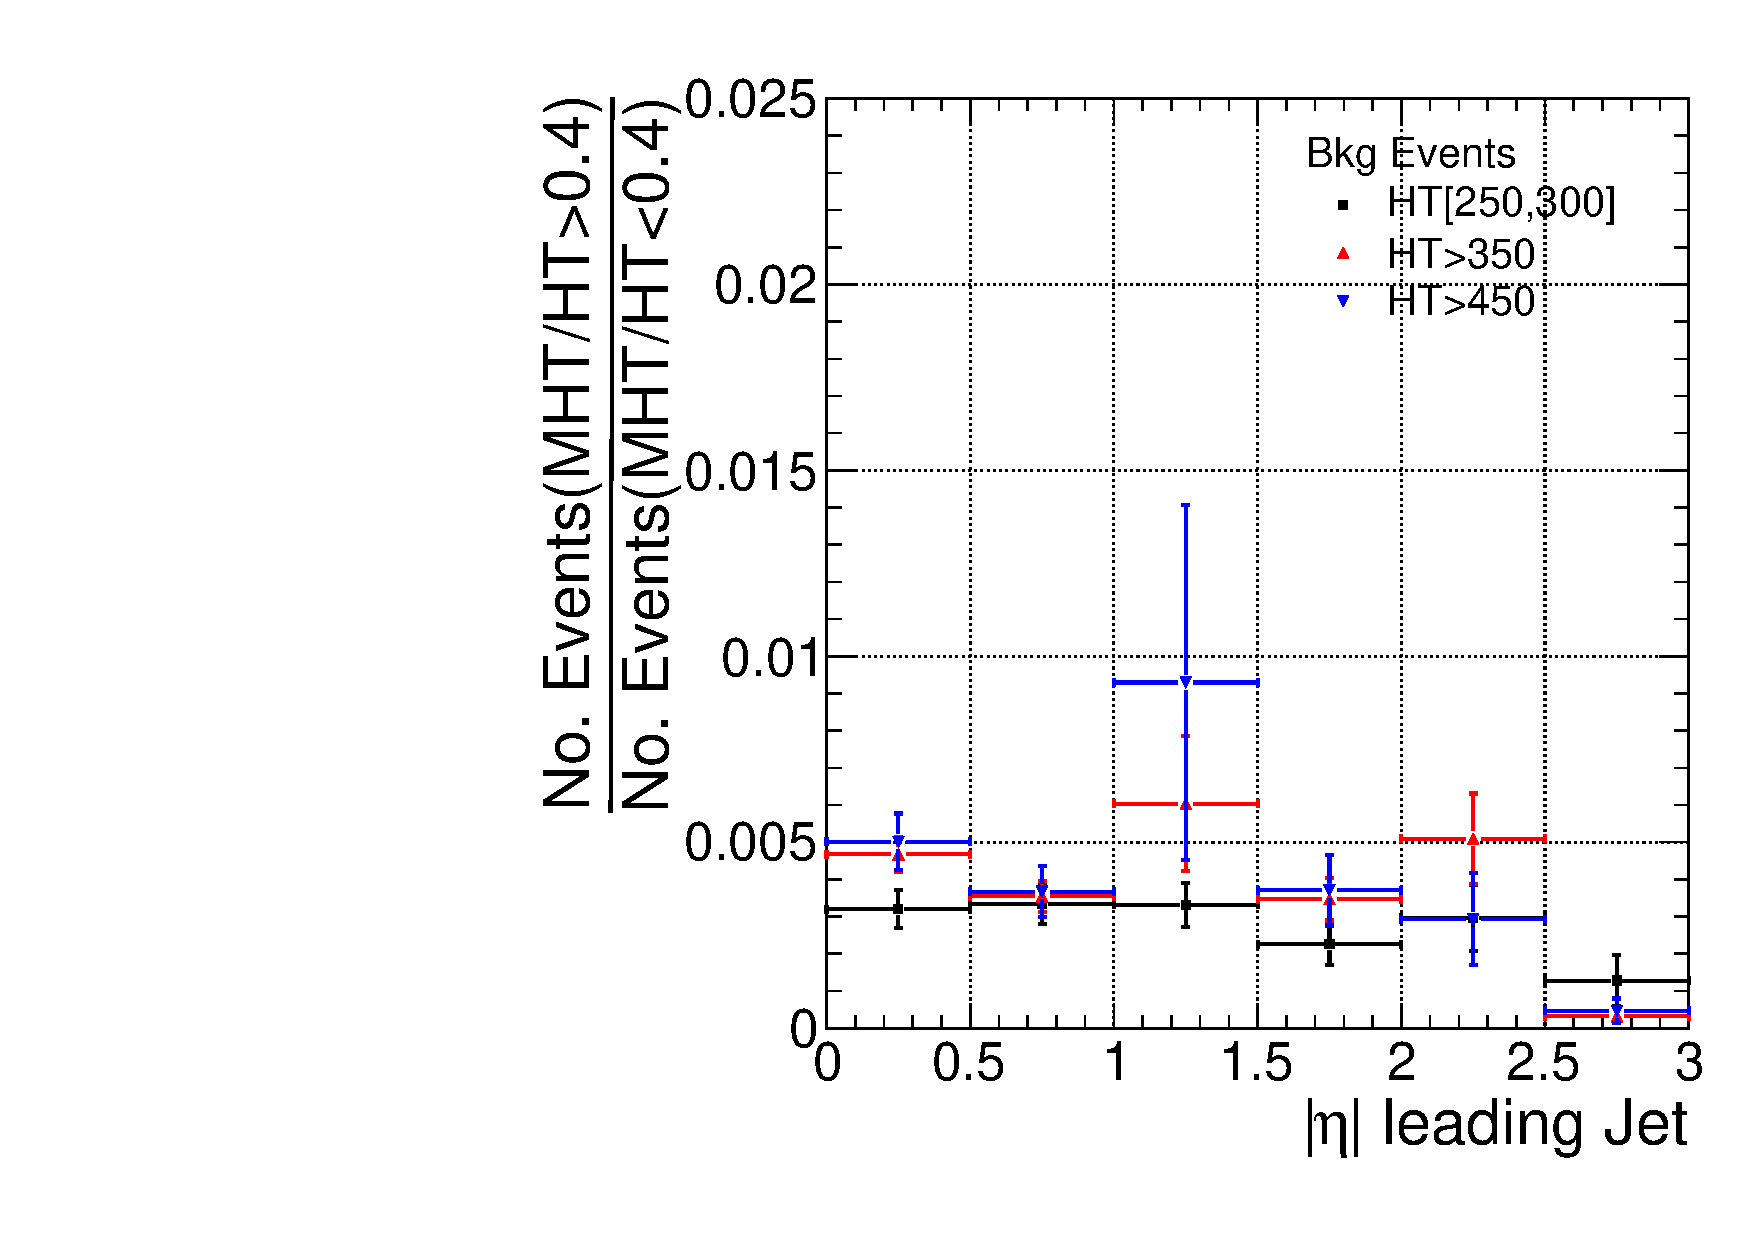
\includegraphics[scale=0.4]{./plots/MHTovHT-NT7-Bkg-MCerr}
%\end{minipage}
%\hspace{0.1cm} % To get a little bit of space between the figures
%\begin{minipage}[b]{0.5\linewidth}
%\centering
%\includegraphics[scale=0.4]{}
%\end{minipage}
\caption{\textit{The $R_{MHT/HT}$ versus the leading jet $|\eta|$ for the SM background-only hypothesis, in three $H_{T}$ bins [250, 350], [350, inf], [450, inf].} }
\label{fig:app3}
\end{figure}

\begin{figure}[h!]
\begin{minipage}[b]{0.5\linewidth}
\centering
{\label{fig:aT}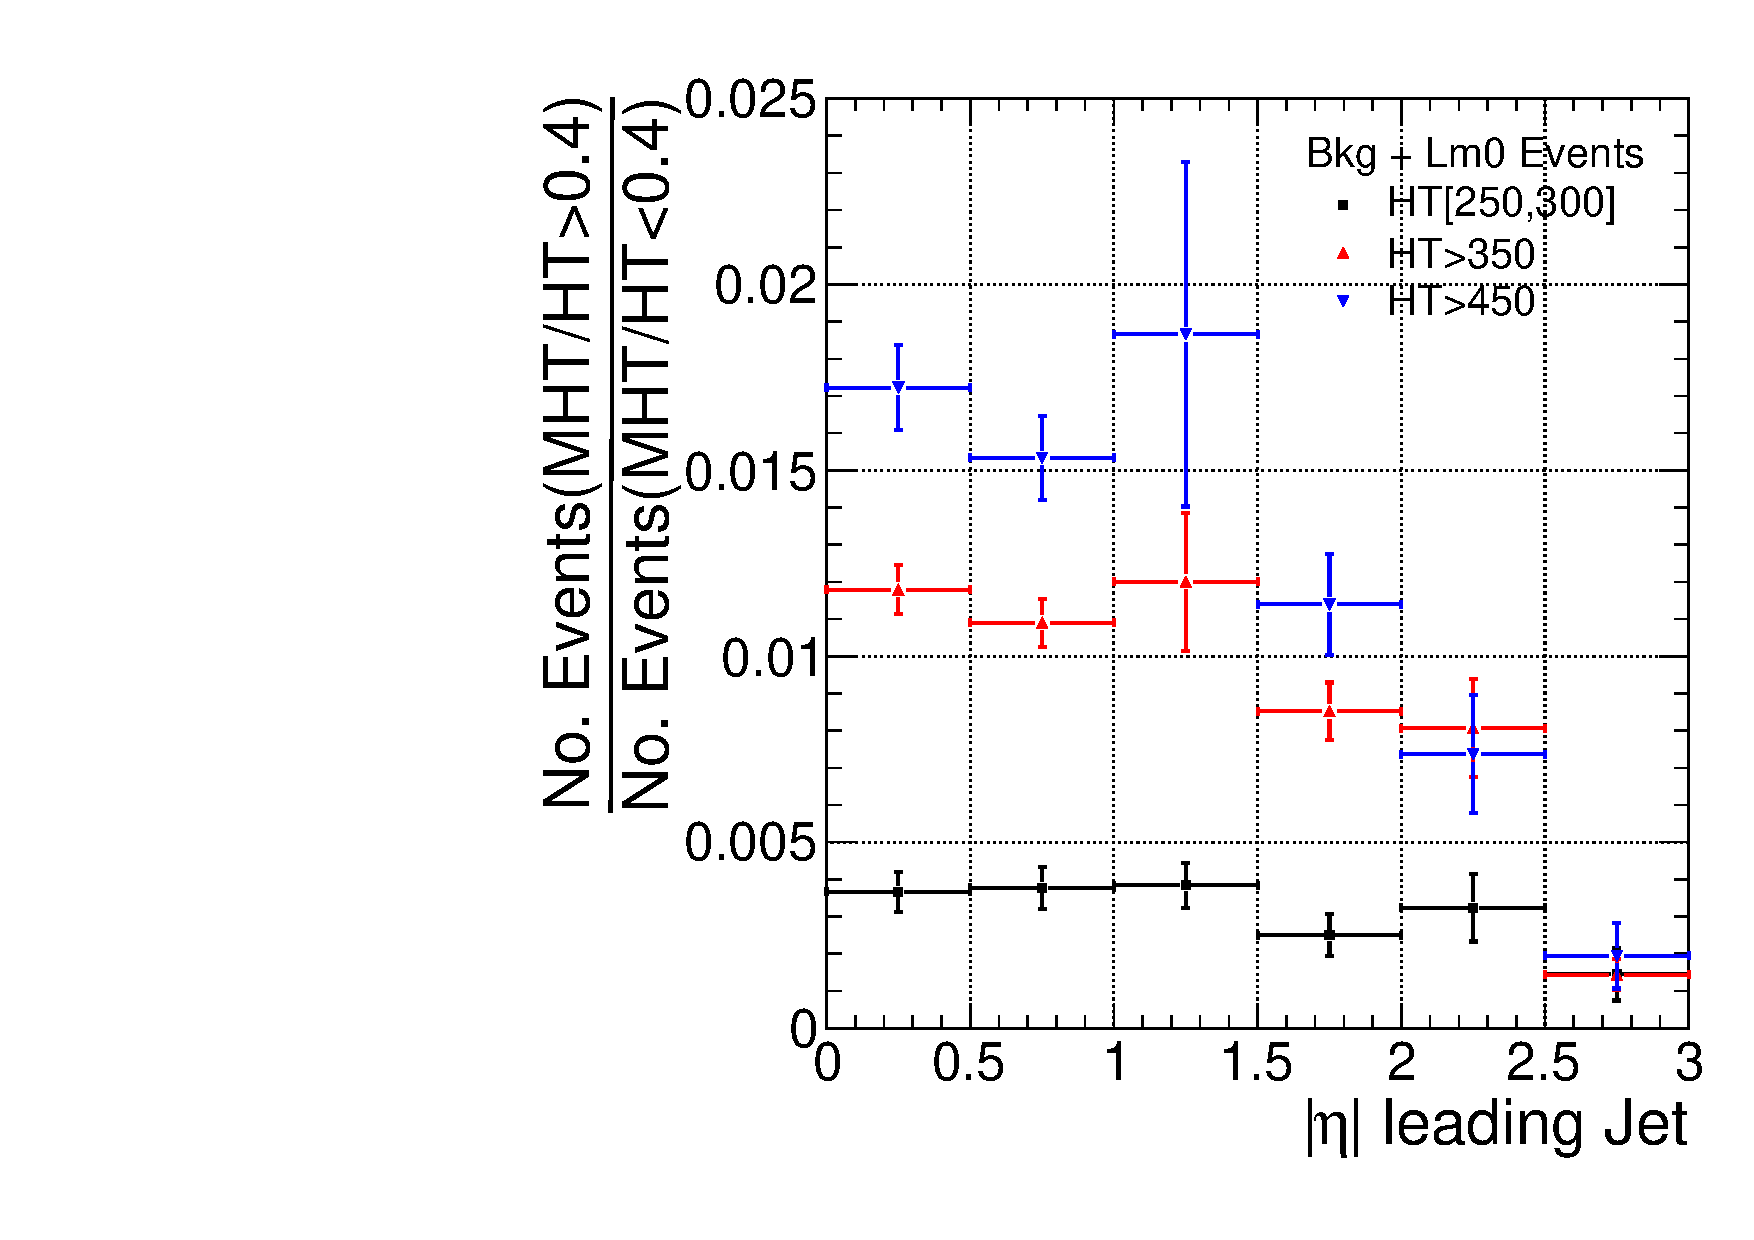
\includegraphics[scale=0.4]{./plots/MHTovHT-NT7-Lm0-MCerr}} 
\end{minipage}
\begin{minipage}[b]{0.5\linewidth}
\centering
{\label{fig:mht}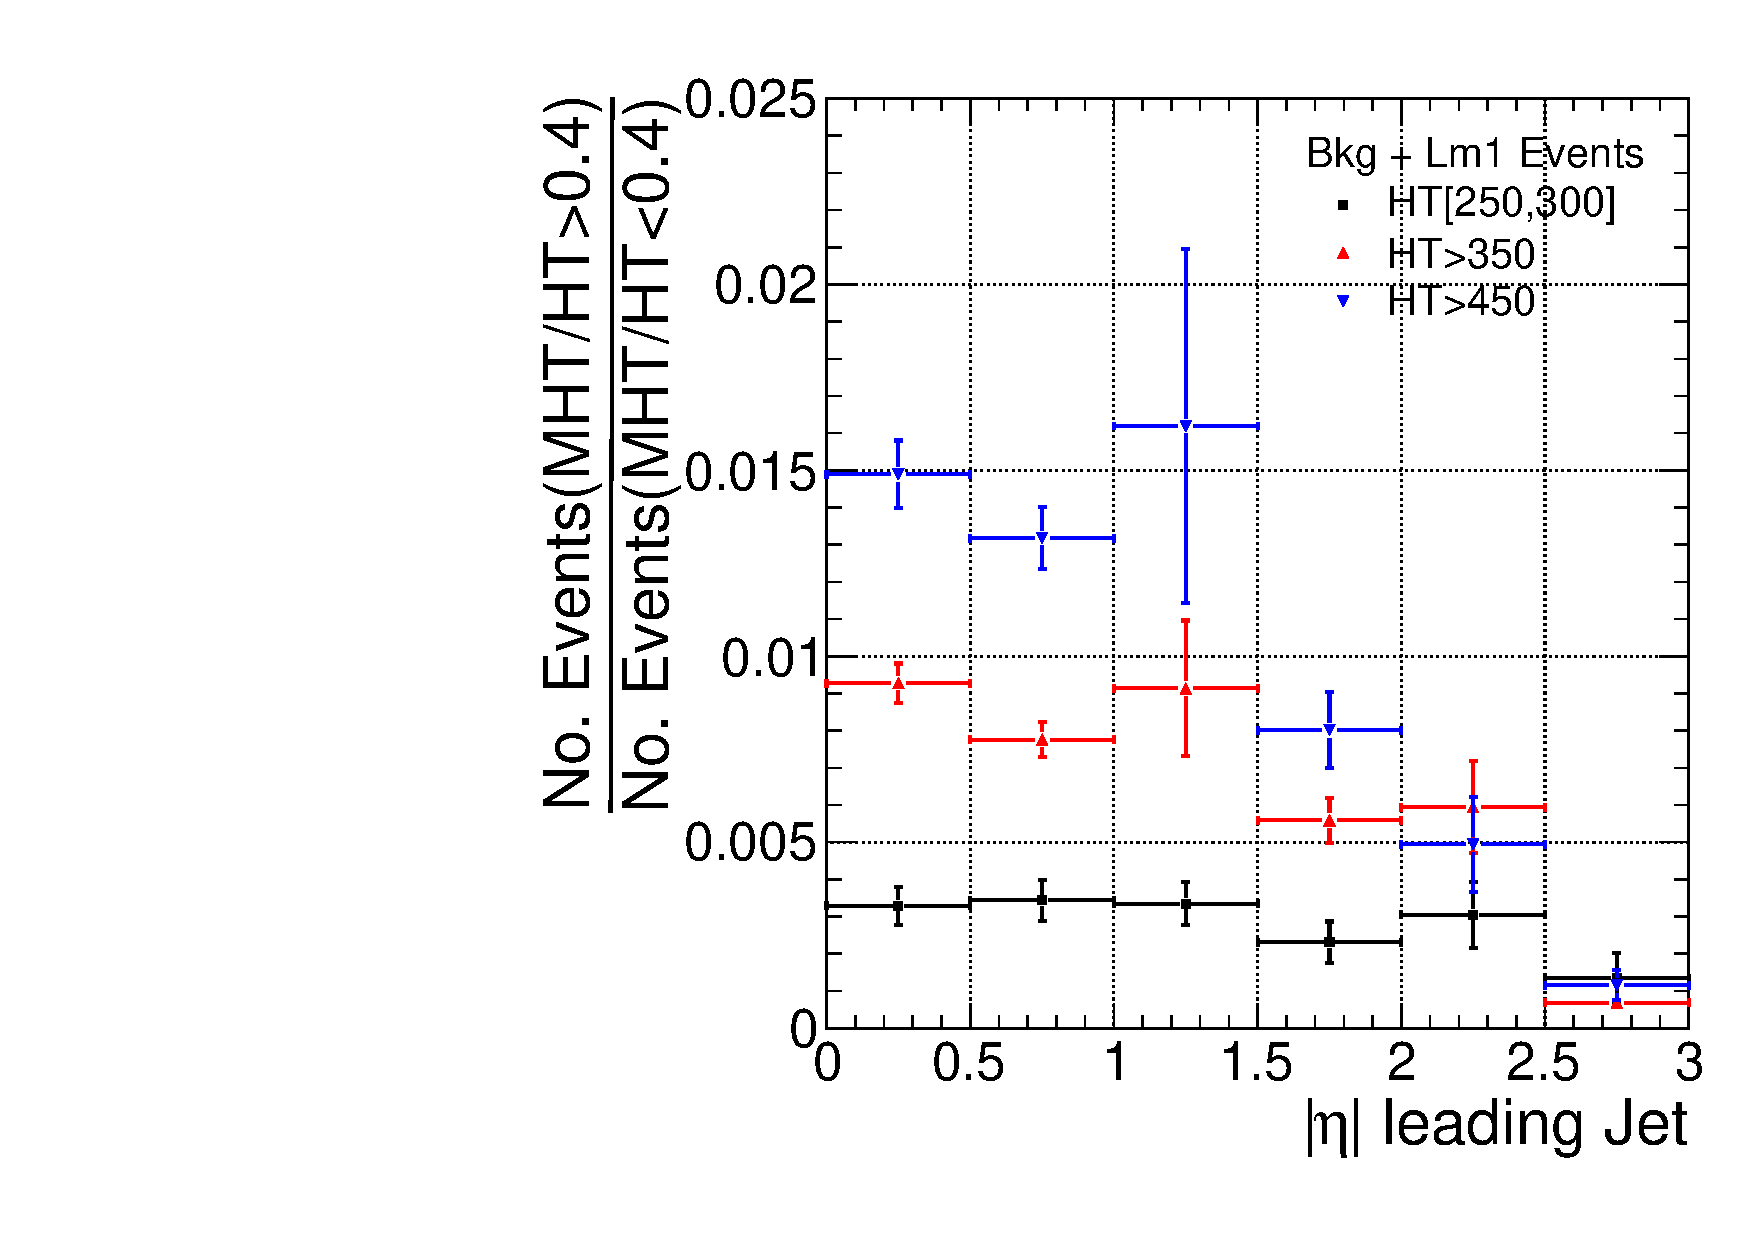
\includegraphics[scale=0.4]{./plots/MHTovHT-NT7-Lm1-MCerr}} 
\end{minipage}
\caption{\textit{The $R_{MHT/HT}$ versus the leading jet $|\eta|$ for the SUSY signal plus SM background hypothesis, in three $H_{T}$ bins [250, 350], [350, inf], [450, inf].} }
\label{fig:app4}
\end{figure}

\begin{comment}
\begin{figure}[h!]
%\begin{minipage}[b]{0.5\linewidth} % A minipage that covers half the page
\centering
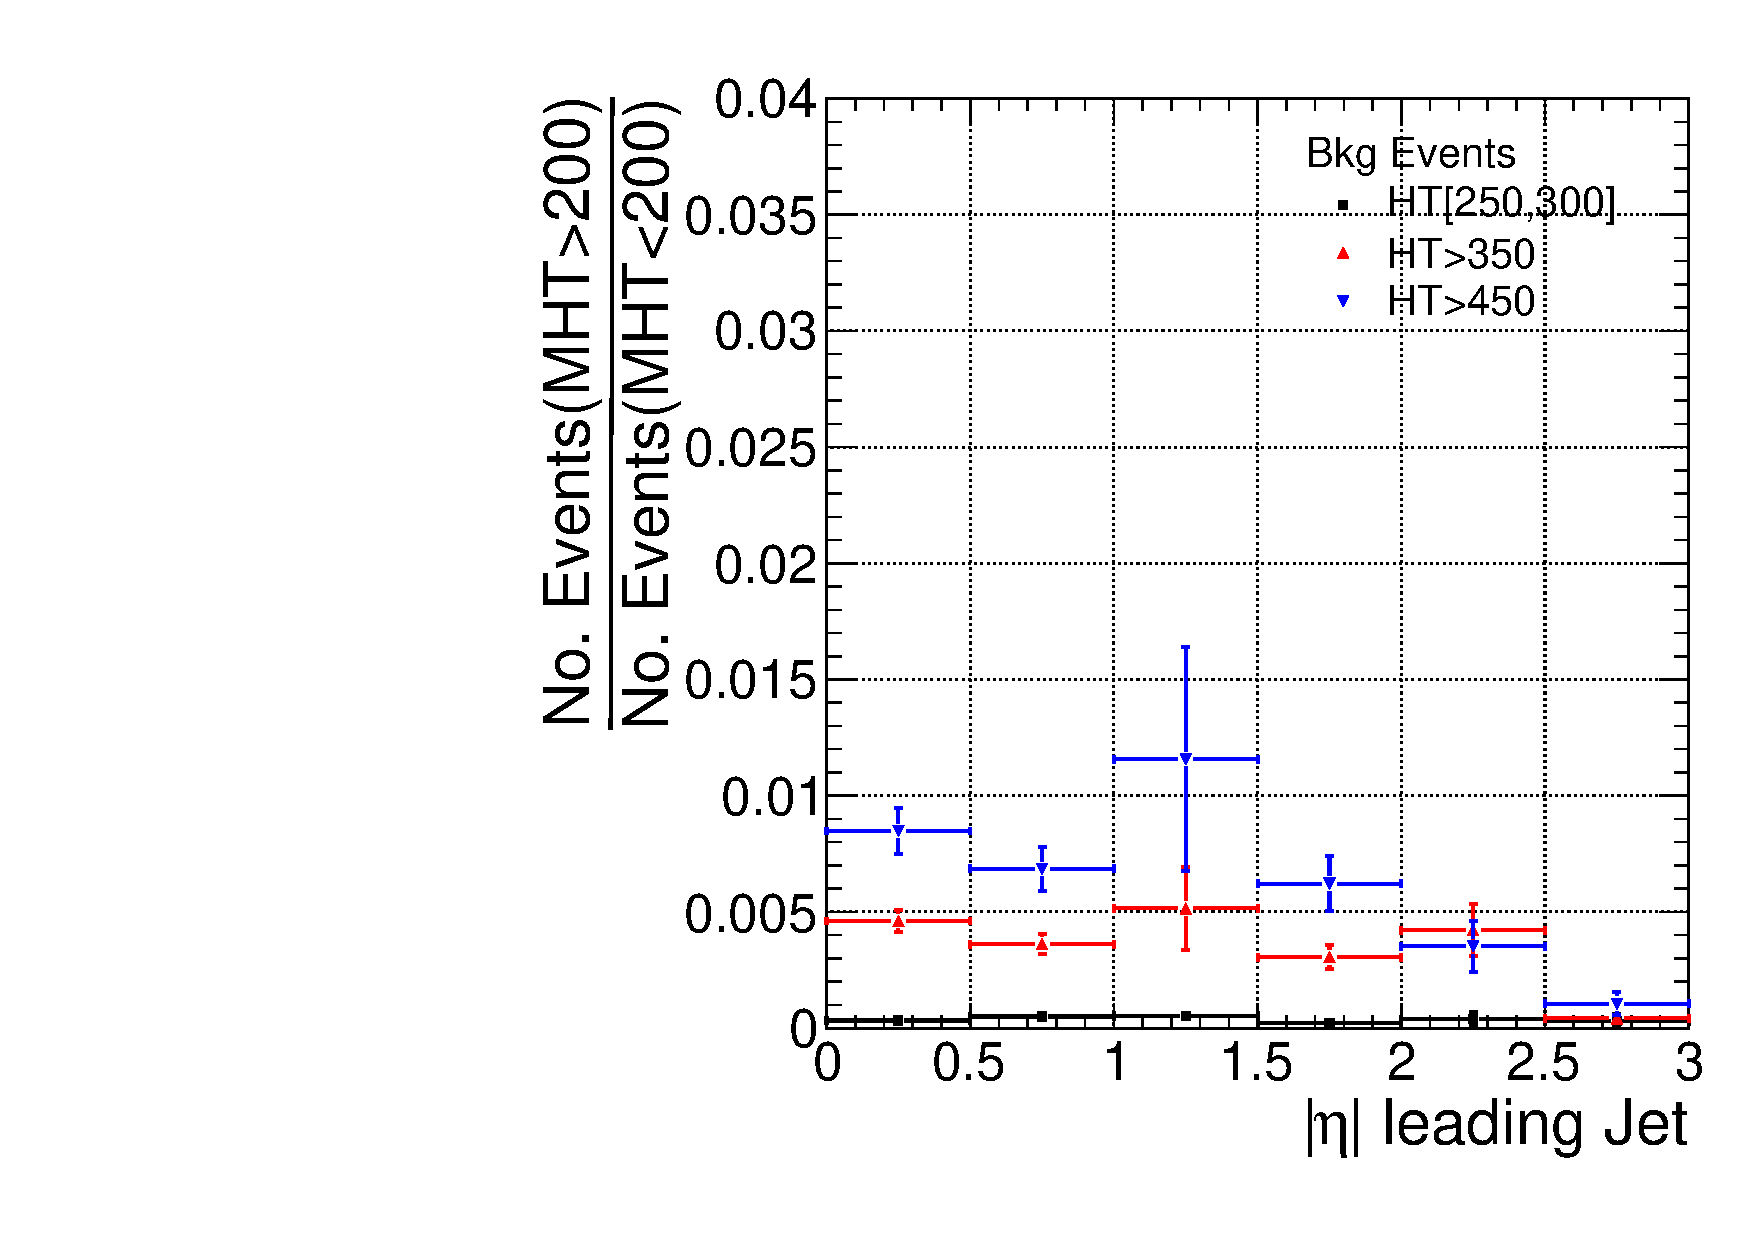
\includegraphics[scale=0.4]{./plots/MHT-NT7-Bkg-MCerr}
%\end{minipage}
%\hspace{0.1cm} % To get a little bit of space between the figures
%\begin{minipage}[b]{0.5\linewidth}
%\centering
%\includegraphics[scale=0.4]{}
%\end{minipage}
%  \caption{ }
\label{fig:app6}
\end{figure}
\begin{figure}[h!]
\begin{minipage}[b]{0.5\linewidth} % A minipage that covers half the page
\centering
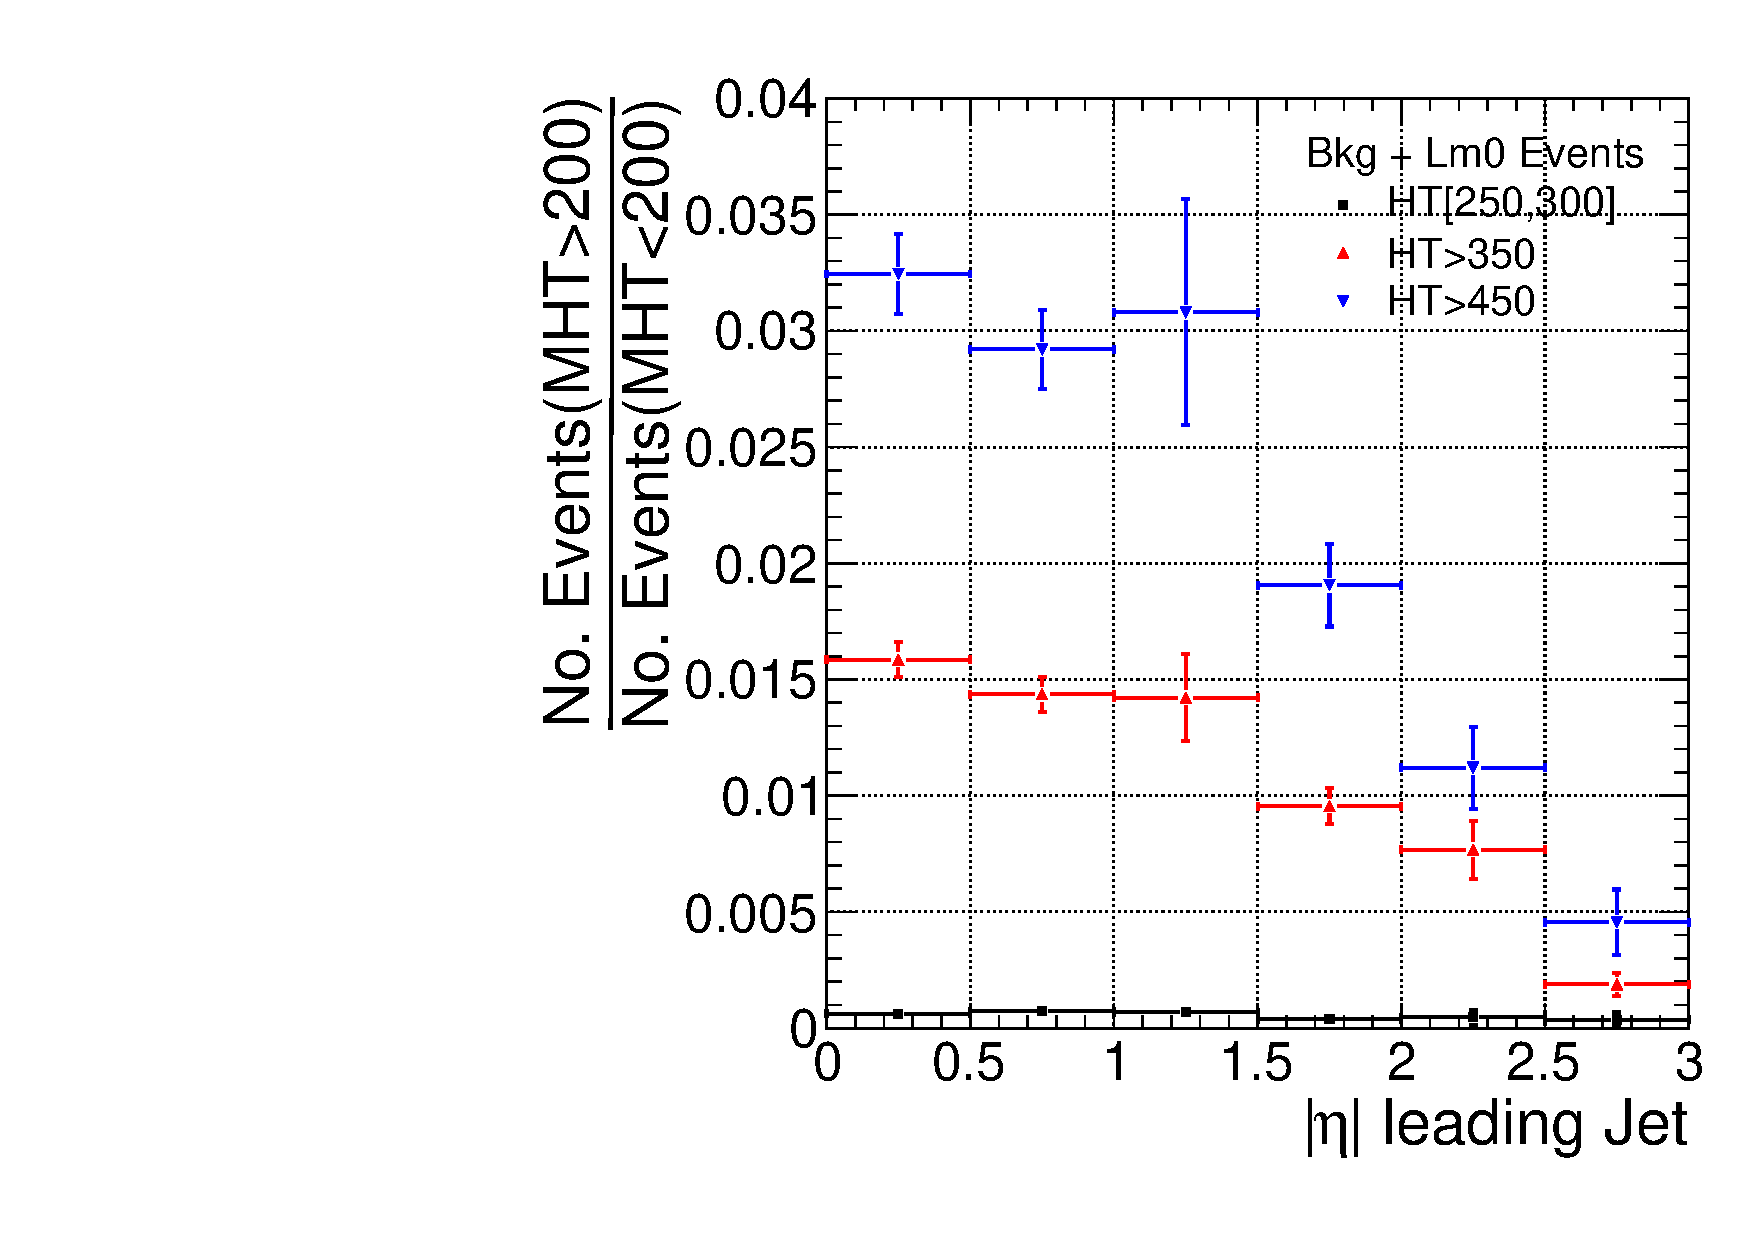
\includegraphics[scale=0.4]{./plots/MHT-NT7-Lm0-MCerr}
\end{minipage}
\hspace{0.1cm} % To get a little bit of space between the figures
\begin{minipage}[b]{0.5\linewidth}
\centering
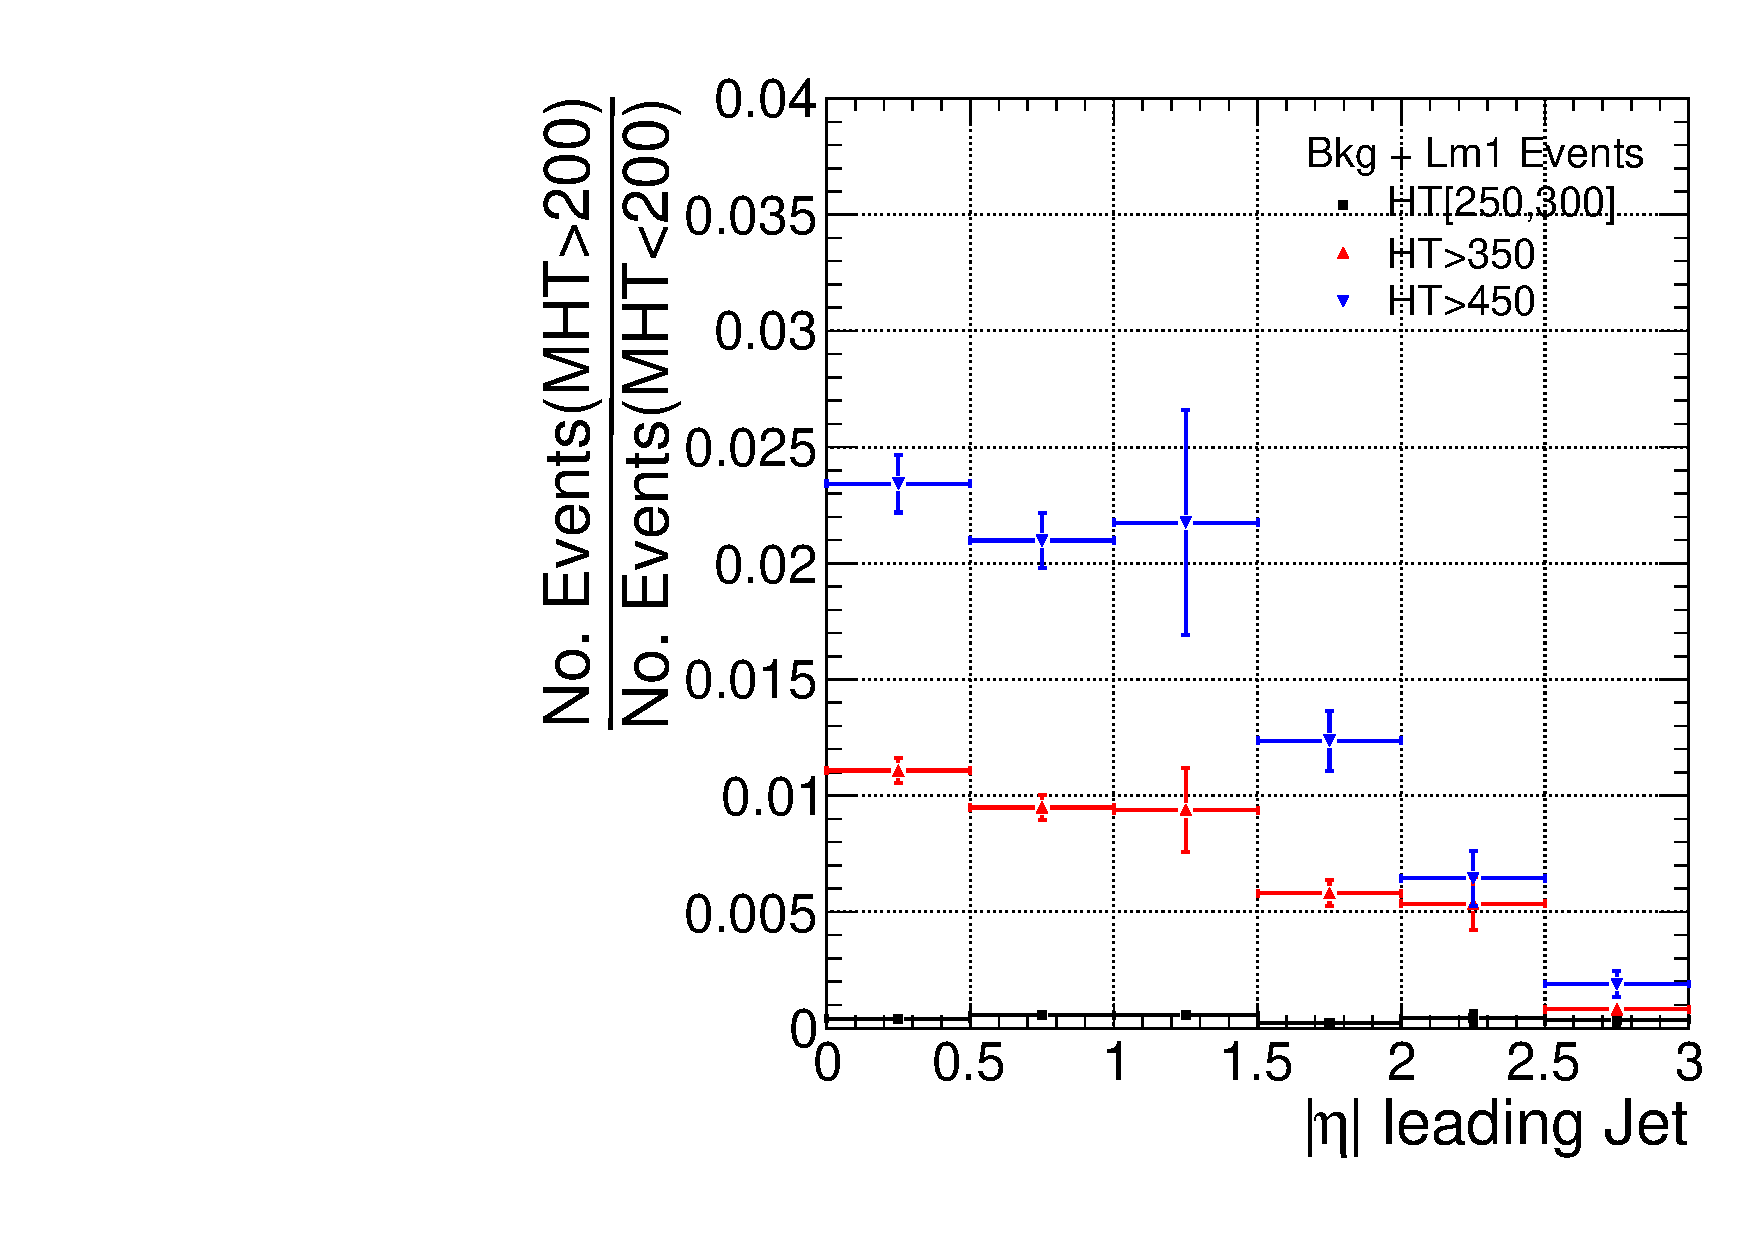
\includegraphics[scale=0.4]{./plots/MHT-NT7-Lm1-MCerr}
\end{minipage}
%  \caption{ }
\label{fig:app4}
\end{figure}

\clearpage
\begin{figure}[h!]
%\begin{minipage}[b]{0.5\linewidth} % A minipage that covers half the page
\centering
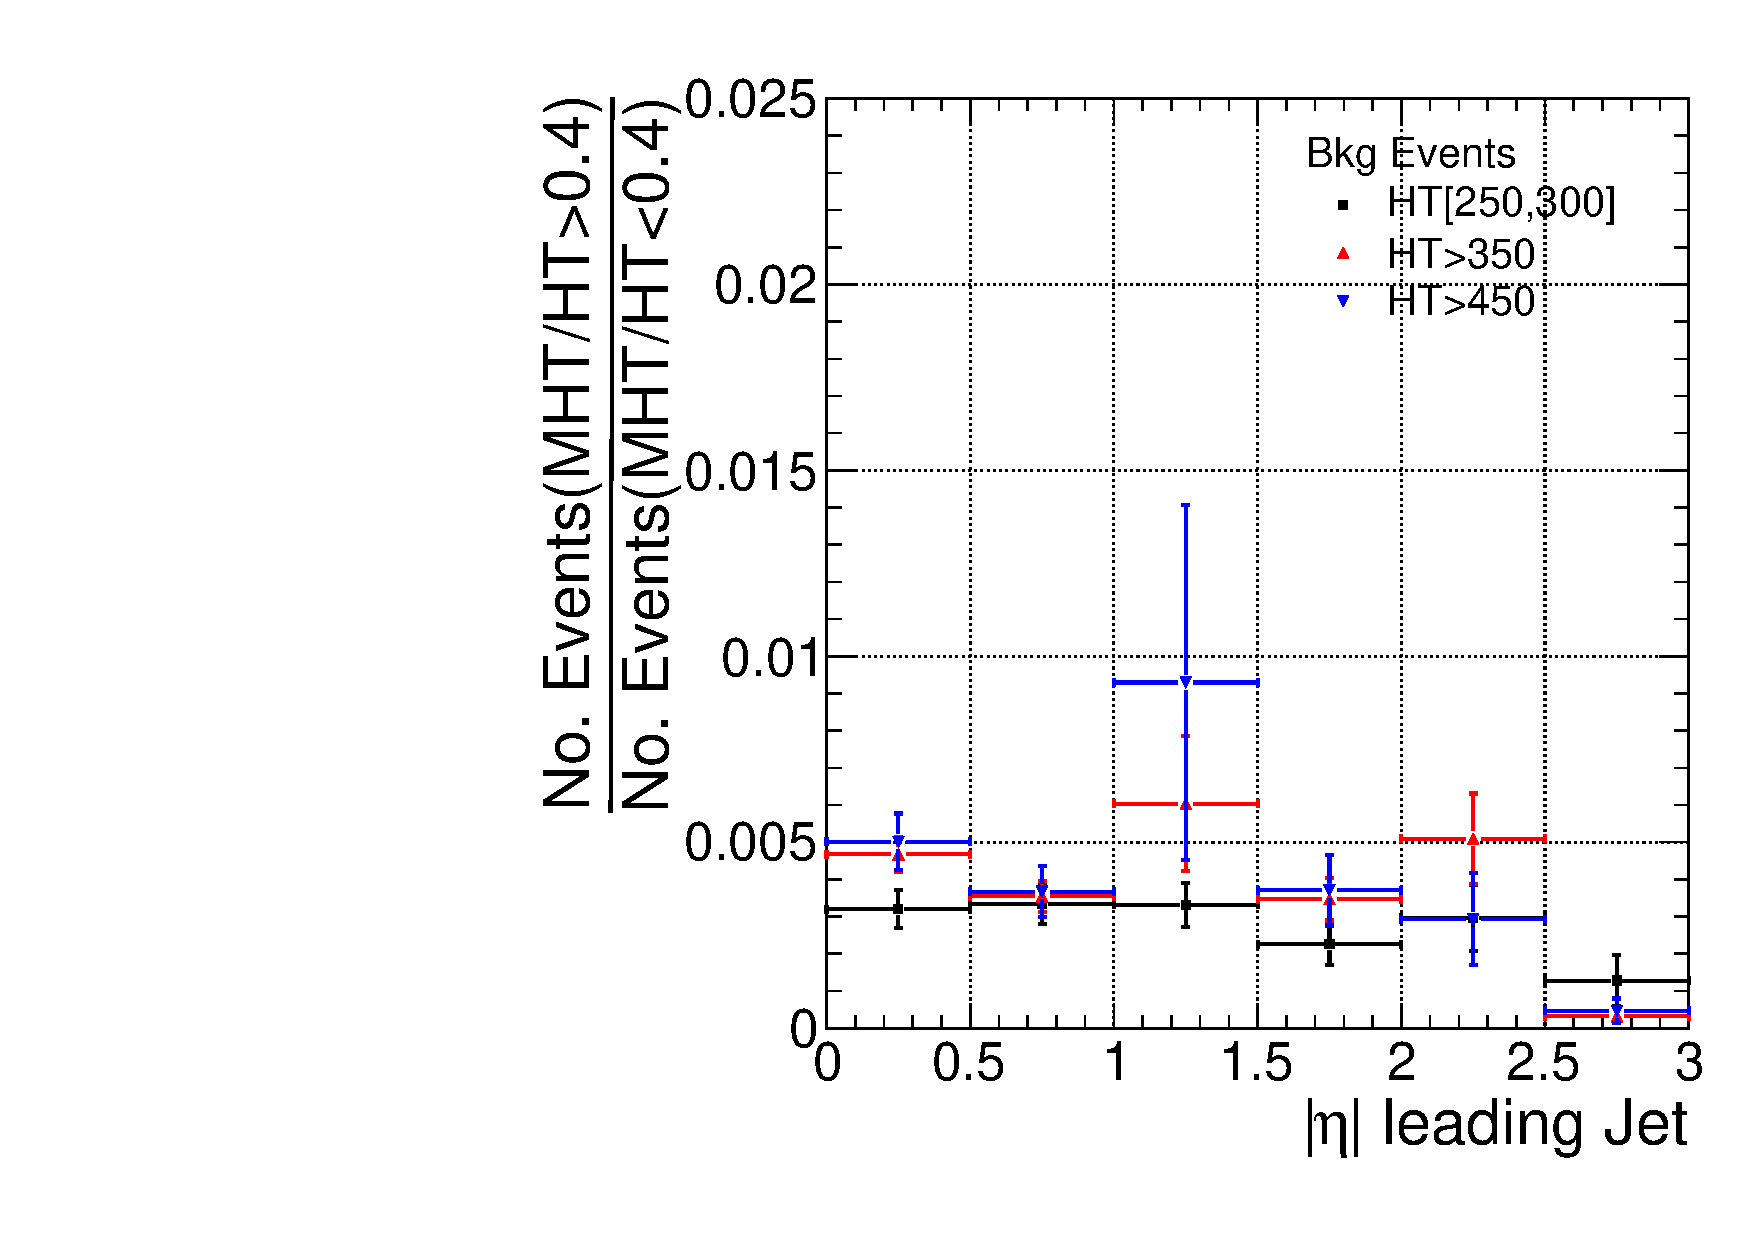
\includegraphics[scale=0.4]{./plots/MHTovHT-NT7-Bkg-MCerr}
%\end{minipage}
%\hspace{0.1cm} % To get a little bit of space between the figures
%\begin{minipage}[b]{0.5\linewidth}
%\centering
%\includegraphics[scale=0.4]{}
%\end{minipage}
%  \caption{ }
\label{fig:id1}
\end{figure}
\begin{figure}[h!]
\begin{minipage}[b]{0.5\linewidth} % A minipage that covers half the page
\centering
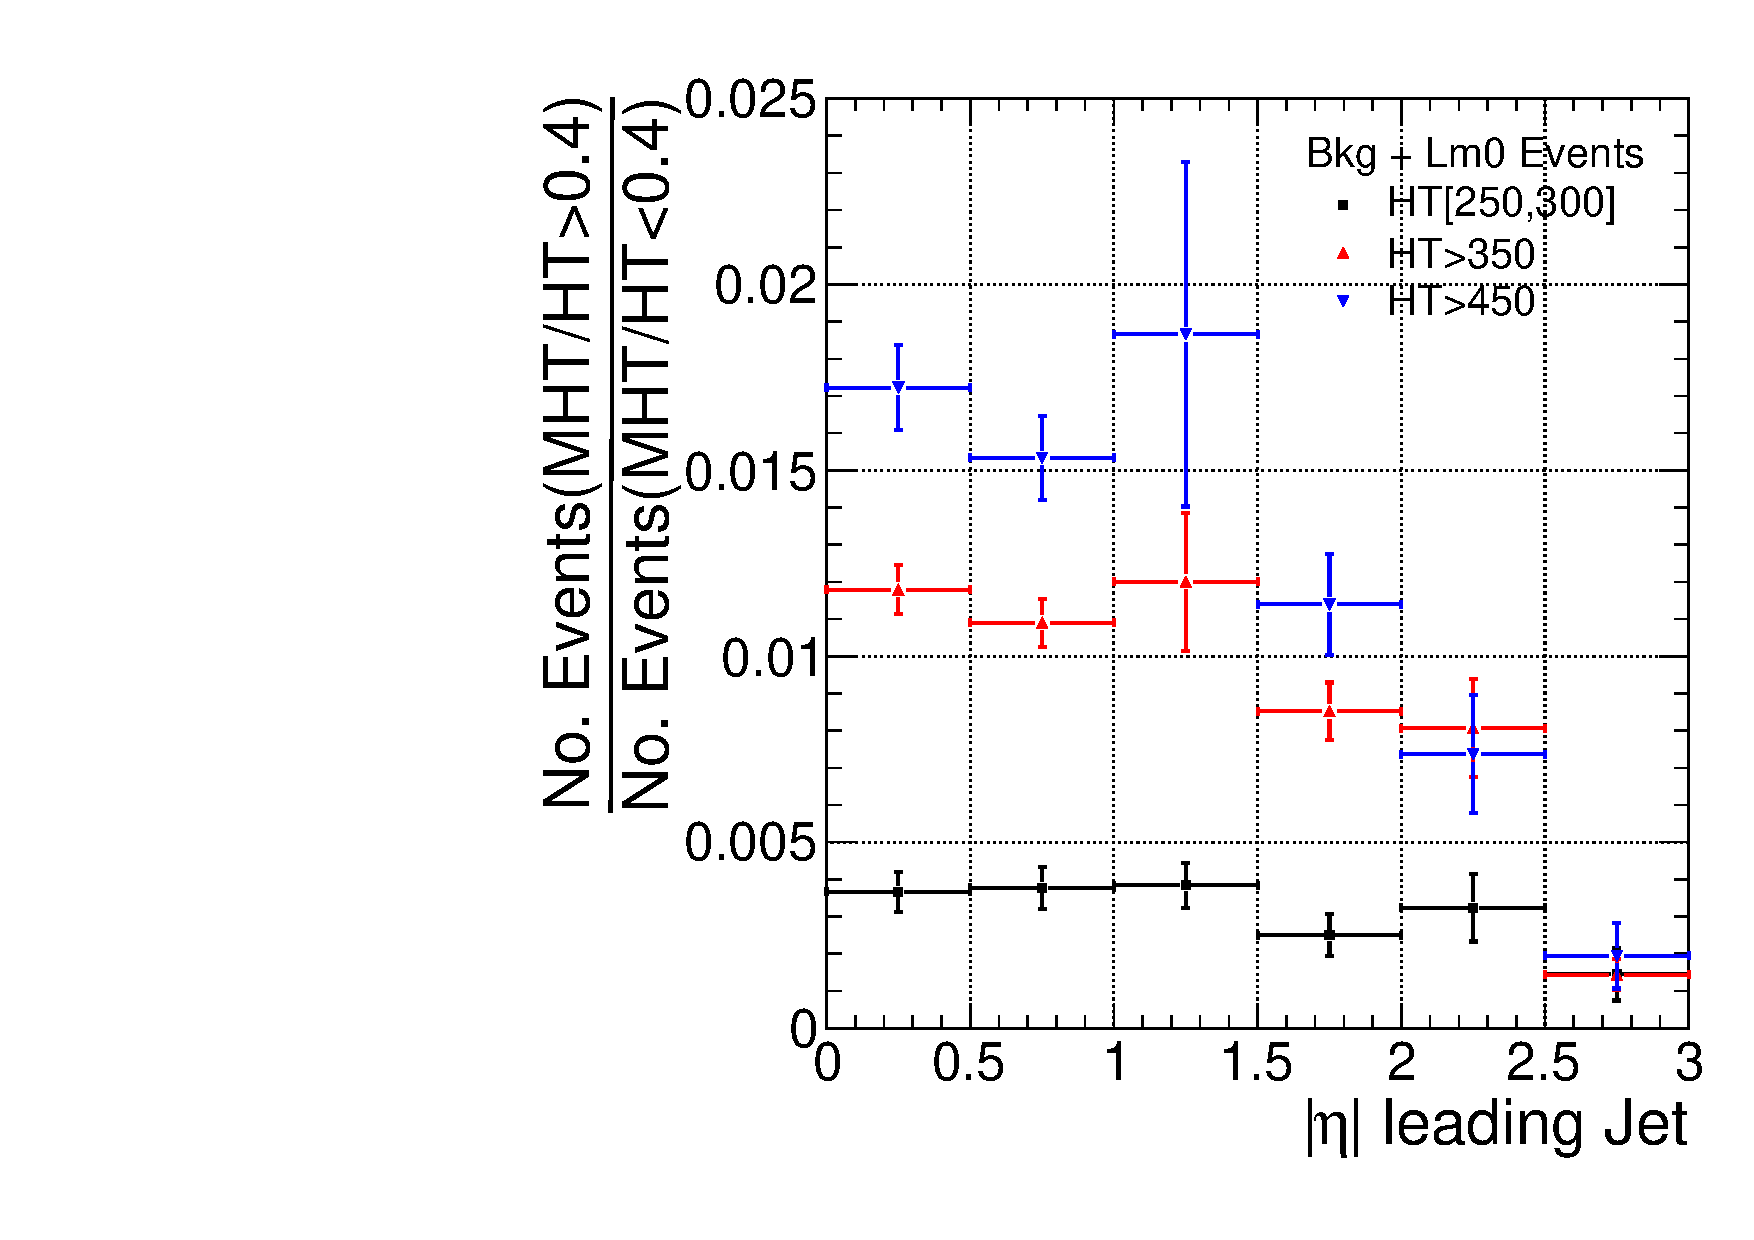
\includegraphics[scale=0.4]{./plots/MHTovHT-NT7-Lm0-MCerr}
\end{minipage}
\hspace{0.1cm} % To get a little bit of space between the figures
\begin{minipage}[b]{0.5\linewidth}
\centering
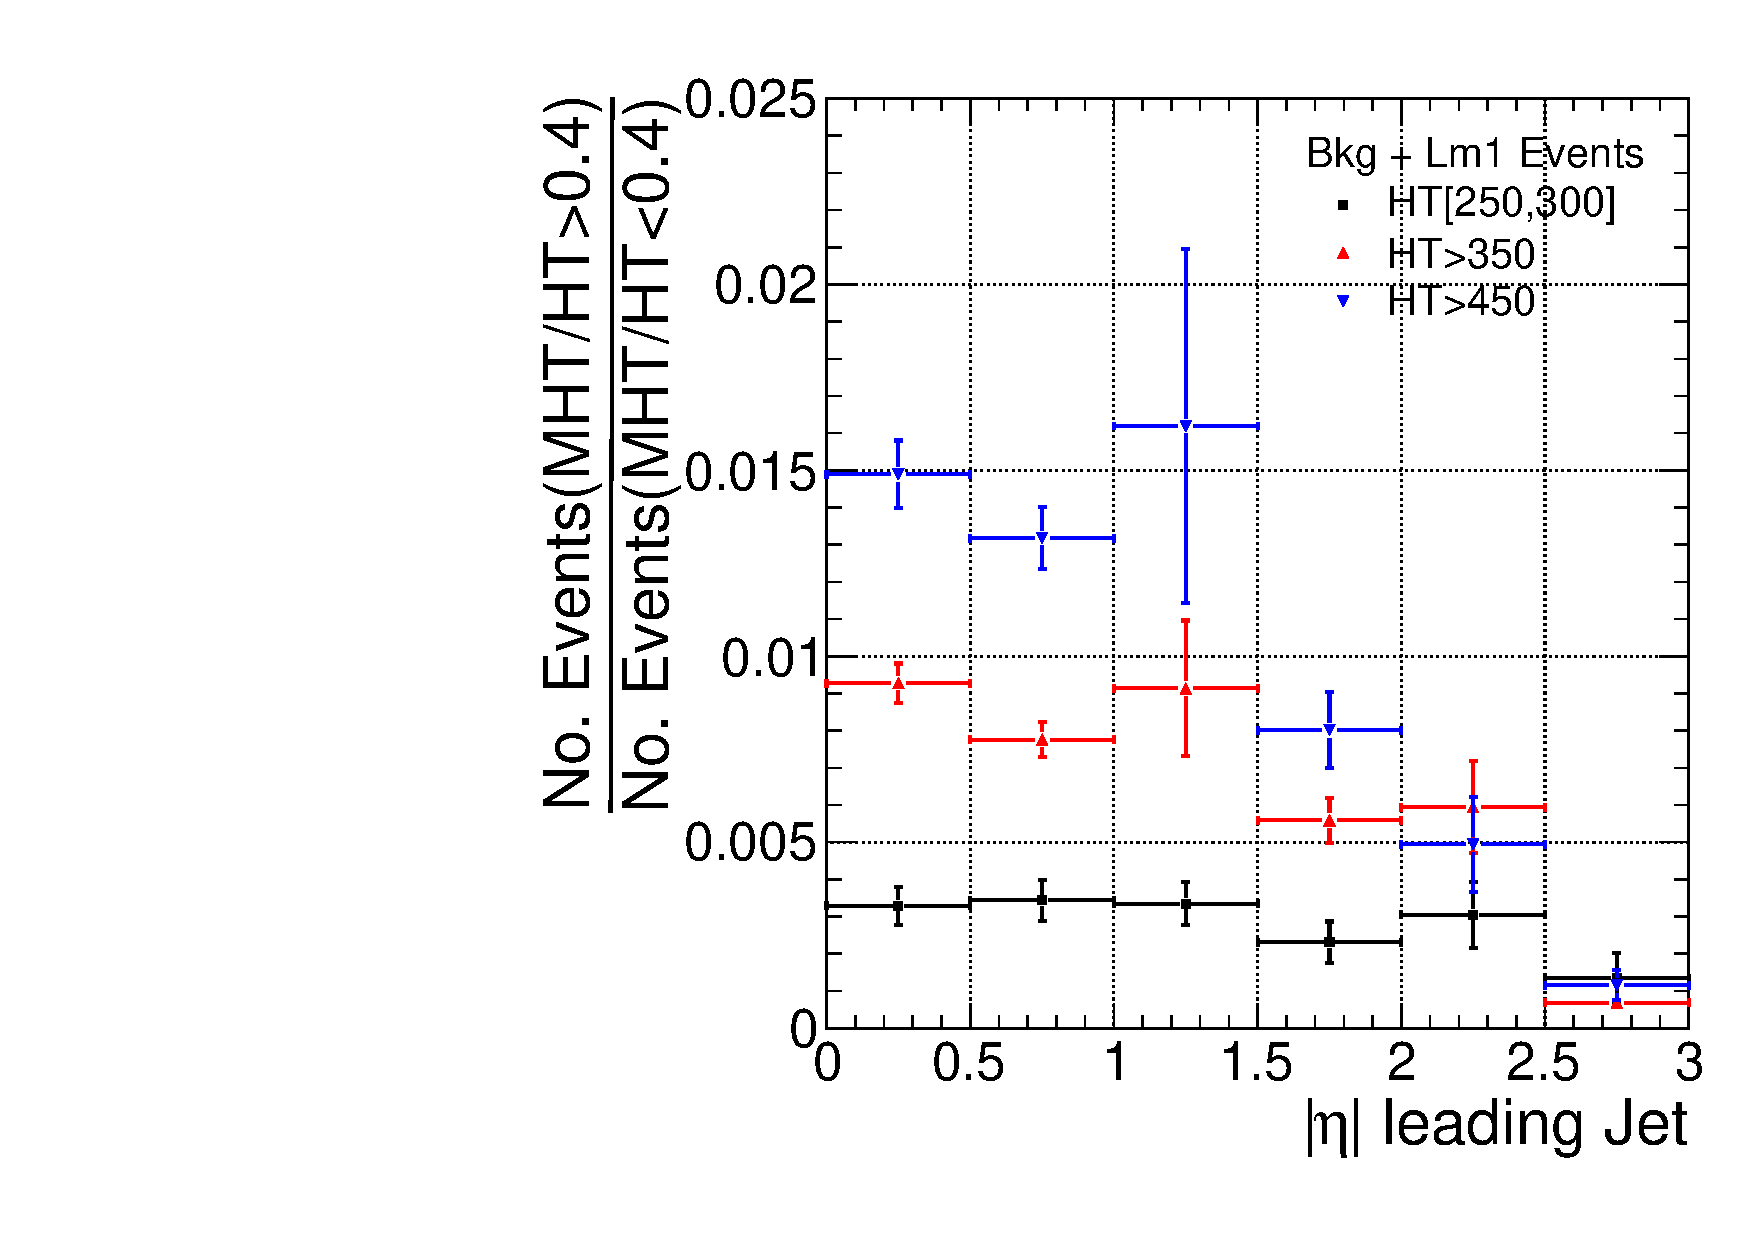
\includegraphics[scale=0.4]{./plots/MHTovHT-NT7-Lm1-MCerr}
\end{minipage}
%  \caption{ }
\label{fig:app5}
\end{figure}
\end{comment}
